\section{Анализ предметной области}
\subsection{Особенности интернет-торговли растениями}

Продажа семян и саженцев по почте — это удобный и популярный способ покупки в России. Больше не нужно обходить множество магазинов в поисках нужных сортов и гибридов: покупатели могут спокойно и внимательно изучить каталог или сайт интернет-магазина, не выходя из дома.

Во многих регионах страны выбор семян и посадочного материала ограничен, а качество и ассортимент уступают тем, что представлены в крупных интернет-магазинах и каталогах компаний. Поэтому жители регионов часто заказывают товары по почте, так как не могут найти нужный сорт или вид растения в обычных магазинах.

Дистанционная торговля семенами и посадочным материалом может осуществляться двумя способами: через каталоги и через интернет-магазины. До недавнего времени основным видом торговли была продажа через каталоги. С развитием интернета в нашей стране, на смену этому виду торговли пришла торговля через интернет-магазины.

Самый популярный и простой товар с точки зрения хранения и доставки — это семена \cite{krivko}. Их можно заказывать круглый год, многие огородники планируют свои посевы ещё с осени и делают заказы заранее, в октябре-декабре. Такие посылки приходят адресату до Нового года. Однако пик заказов обычно приходится на январь-февраль. Заказывая семена, всегда нужно учитывать сроки посева каждой культуры. Затем отнимается 3-5 дней на комплектацию заказа и 5-20 дней на доставку почтой, в зависимости от региона. В итоге получается, что заказ семян следует делать минимум за месяц до посева \cite{kaygorodtseva}.

Второй по популярности товар — это луковичные и многолетние растения. Этот вид товара имеет два сезона продаж — весна и осень. Весной предлагается огромный ассортимент многолетних растений, таких как астильбы, хосты, пионы травянистые, гейхеры, а также луковичных растений, таких как гладиолусы, лилии, амариллисы. Срок приёмки заказов с ноября по апрель, отправка заказов начинается в марте. Осенний сезон более короткий и предлагает тюльпаны, нарциссы, крокусы, гиацинты и различные мелколуковичные растения. Заказы принимаются с июля по август, отправка осуществляется с августа по сентябрь.

Саженцы плодовых и декоративных кустарников и деревьев — следующий по популярности товар. Приём заказов начинается с ноября, а рассылка стартует после 8 марта.

Саженцы кустарников и деревьев, а также луковичные и многолетние растения — это более специфический продукт, чем семена. Для сохранения качества им нужны определённые температурные условия.
При выборе оплаты наложенным платежом покупатель оплачивает посылку при получении на почте. Стоимость посылки состоит из нескольких компонентов: стоимости товара, стоимости доставки, которая зависит от веса посылки, расстояния и выбранного способа доставки, а также комиссии за обработку наложенного платежа, которую взимает почтовая служба или курьерская компания.

При выборе предоплаты покупатель заполняет квитанцию в каталоге или получает её на электронную почту. Отправка заказа осуществляется после поступления денег на расчётный счёт продавца. При получении товара на почте покупатель оплачивает только расходы за почтовую пересылку.


\subsection{Характеристики растений}

При неправильном уходе растения могут погибнуть, это уменьшит доверие покупателей к интернет-магазину. Поэтому на сайте необходимо разместить советы по выращиванию того или иного растения. Для этого требуется изучить их характеристики и вытекающие из них классификации. Указание декоративных характеристик растений также упростит пользователю выбор товара и принесёт больше положительных эмоций от пользования сайтом.

Декоративные растения — это разнообразная группа растений, включающая как культивируемые, так и дикие виды деревьев, кустарников, многолетних и однолетних растений, злаков и луковичных растений, которые принадлежат к различным ботаническим семействам. 

Декоративные злаки — это растения семейства злаковых, которые используются для создания групповых посадок и бордюров, газонов, а также для составления букетов. Они обладают привлекательной текстурой и формой, что делает их популярными элементами ландшафтного дизайна \cite{kingsberry}.

Луковичные растения представляют собой обширную группу декоративных растений, различающихся по цвету, размеру, форме цветков и времени цветения. В открытом грунте они цветут с весны до осени, а благодаря зимней выгонке способны цвести практически круглый год. Эти растения могут использоваться для выращивания в помещении и для создания букетов. С точки зрения распространения по миру, луковичные растения представляют одну из самых многочисленных групп. Они включают в себя преимущественно лилейные и амариллисовые семейства \cite{belyaevskaya}.

На примере луковичных растений хорошо заметна разница требований разных растений к почве. Для лилий подходят лёгкие глинистые почвы с хорошей дренажной системой, практически без извести. Гиацинты и тюльпаны предпочитают песчаные почвы, богатые питательными веществами, с нейтральной кислотностью. Тяжёлые глинистые почвы с плохой водопроницаемостью, а также очень бедные песчаные почвы не подходят для луковичных растений \cite{doroshenko}.

Декоративные деревья и кустарники бывают хвойные и лиственные, вечнозелёные или с опадающей листвой. Их красота зависит от внешних характеристик, таких как форма кроны, цвет и структура листьев, а также цвет и размер цветов и плодов. Подходящие условия для роста помогают сохранить красоту растений, которая меняется вместе с возрастом и сменой времен года в зависимости от генетических особенностей вида.

У декоративных растений существуют два способа размножения: семенной и вегетативный. Вегетативное размножение деревьев и кустарников осуществляется через черенки, отводки, корневые отпрыски, прививки или деление куста \cite{berd}.

Жизненный цикл декоративных растений — это онтогенез, или индивидуальное развитие растения от его появления из оплодотворенной яйцеклетки или вегетативной почки (черенка с почками, корневого отпрыска и т.п.) до отмирания. По продолжительности жизненного цикла растения подразделяются на однолетние, двулетние и многолетние.

\subsubsection{Многолетние растения}

Характерной чертой многолетних травянистых растений является способность переживать зиму на открытой земле, ежегодно проходить через все стадии развития (рост, цветение, плодоношение) и продолжать этот цикл на протяжении многих лет благодаря специальным органам, предназначенным для зимовки (корень, корневище, луковица, ползучие стебли и другие).

У большинства декоративных многолетников надземная часть каждый год отмирает, но на следующий сезон восстанавливается за счет измененного подземного стебля в виде корневищ, луковиц, клубнелуковиц (например, луковичные растения, пионы, флоксы, рудбекия, акониты и другие) \cite{viyginaOpen}.

У других растений надземные побеги не отмирают, а сохраняются зимой, когда все жизненные процессы, как у древесных растений, замедляются. С приходом весны и благоприятных условий из почек начинают развиваться новые вегетативные и генеративные побеги, которые цветут и образуют семена.

У некоторых видов растений стебель и корень, помимо своих основных функций, также выполняют задачи вегетативного размножения и защиты растений зимой.

Существуют три основных типа подземных стеблей: луковица, клубень (клубнелуковица) и корневище.

Луковица – это видоизменённый побег с плотным коротким стеблем и мясистыми листьями, имеющими вид чешуек и запасающими воду и питательные вещества \cite{belyaevskaya}.

Клубень -- это укороченный, значительно утолщенный подземный побег, который запасает питательные вещества. Клубни, имеющие форму луковицы, называются клубнелуковицами.

Корневище -- это долговечное стеблевое образование, внешне напоминающее корень, но отличающееся наличием дополнительных корней и почек. На его поверхности можно видеть следы прикрепления листьев в виде коричневых чешуек и остатки умерших побегов. Корневище может быть горизонтальным, утолщенным (как у ириса, бадана, ландыша), растущим вертикально или наклонно вниз (как у астильбы, примулы, функии, диклитры) \cite{aldohina}.

Многолетние растения, благодаря своим биологическим особенностям, способны выдерживать низкие температуры зимой. Молодые экземпляры имеют невысокую степень морозоустойчивости, но по мере их развития эта способность увеличивается. Однако по мере завершения жизненного цикла у растений морозоустойчивость снова снижается. Для сохранения и развития этого ценного биологического свойства растений важна своевременная подготовка к зиме, проведение осенних и ранневесенних посевов в открытый грунт. Не столько низкие температуры, сколько резкие перепады могут нанести вред многолетникам. Особенно опасны для них зимы без снега, с оттепелями и долгими затоплениями поверхности почвы водой. Поэтому для выращивания многолетников, особенно тех, что длительное время находятся на одном месте (например, пионы, флоксы, функии и другие), необходимо выбирать ровные, хорошо дренированные участки без застоя воды.

При создании декоративных миксбордеров (цветников-бордюров из смешанных растений разных размеров и оттенков) важно учитывать морозоустойчивость растений и подбирать ассортимент с учетом конкретных почвенно-климатических условий каждой зоны. Только таким образом можно обеспечить успешное процветание и красоту растений в течение долгого времени \cite{karpisonova}.

\subsubsection{Двулетние растения}

В цветоводстве под двулетниками понимаются растения, которые по своей природе являются многолетниками, но достигают пика декоративного эффекта в период своего второго года жизни. К их числу относятся такие виды, как виола, колокольчики, наперстянка, маргаритки и незабудки.

Двулетники обладают разнообразными биологическими и декоративными характеристиками, благодаря чему их применяют для украшения садов и цветников в начале весны, в качестве материала для создания цветочных композиций, для выращивания в горшках, а также для украшения помещений и пристенного озеленения \cite{aldohinaFlower}.

В отличие от однолетников, двулетники не завершают свой жизненный цикл за один сезон. В первый год они формируют мощную розетку листьев, в то время как во втором году достигают максимального цветущего состояния и дают плоды. В ходе третьего зимнего сезона большая часть растений гибнет, но из семян, оставшихся после увядания, вновь появляются новые растения, которые также достигают пика цветения во втором году своей жизни. Таким образом, участки, занятые двулетниками, способны к самовозобновлению и могут сохранять свою декоративность на протяжении многих лет, со временем изменяя свой облик.

При сильной засухе двулетники могут зацвести и дать небольшое количество семян в первый год жизни.

\subsubsection{Однолетние растения}

К группе однолетников относятся однолетние цветочные культуры, которые проходят все стадии развития за один сезон. Это астры, ноготки, бархатцы, васильки, алиссумы, маки, флоксы летние и другие растения.

В год посева они цветут, дают семена и погибают. Продолжительность их жизни — всего несколько месяцев в году. Однако по разнообразию форм, яркости окраски цветков и длительности цветения многие летники превосходят другие цветочные растения. Они обладают исключительным многообразием по всем декоративным особенностям и предоставляют продолжительное время  для срезки в букеты — от апреля до самых морозов. Кроме того, летники имеют ещё одно положительное свойство — их можно пересаживать в цветущем состоянии.

К однолетникам причисляют некоторые грунтовые многолетники, которые зацветают в первый же год, но не переносят зиму в наших условиях. К ним относятся львиный зев, петуния, вербена и другие растения, которые на своей родине живут по несколько лет.

По декоративным качествам и применению в озеленении летники можно разделить на цветущие и лиственно-декоративные (орнаментальные), бордюрные и вьющиеся.

Большой видовой и сортовой ассортимент однолетних растений позволяет выбрать множество однолетников, которые можно размножать безрассадным способом — посевом семян в открытый грунт \cite{aleksandrova}. Этот способ отличается доступностью и дешевизной.



\subsection{Анализ существующих интернет-магазинов}
\label{shopsAnalize}
Анализ существующих сайтов с похожей тематикой позволяет выделять достоинства и недостатки, чтобы использовать эту информацию для улучшения качества собственной разработки.

Существует большое количество интернет-магазинов декоративных растений. Для анализа были выбраны 3 сайта, занимающие верхние строчки в поисковике <<Яндекс>> при запросе <<Интернет-магазин декоративных растений>>:
\begin{itemize}
	\item <<garshinka>>;
	\item <<pervocvet-shop>>;
	\item <<plantmania>>.
\end{itemize}

Все вышеперечисленные сайты имеют такие базовые страницы, как каталог товаров, корзина покупателя и вход в личный кабинет. Наибольший интерес для анализа вызывает каталог товаров, так как  его структура на разных сайтах отличается.

На рисунке ~\ref{garshinka:image} представлен каталог товаров интернет-магазина <<garshinka>>.

\begin{figure}[h!]
	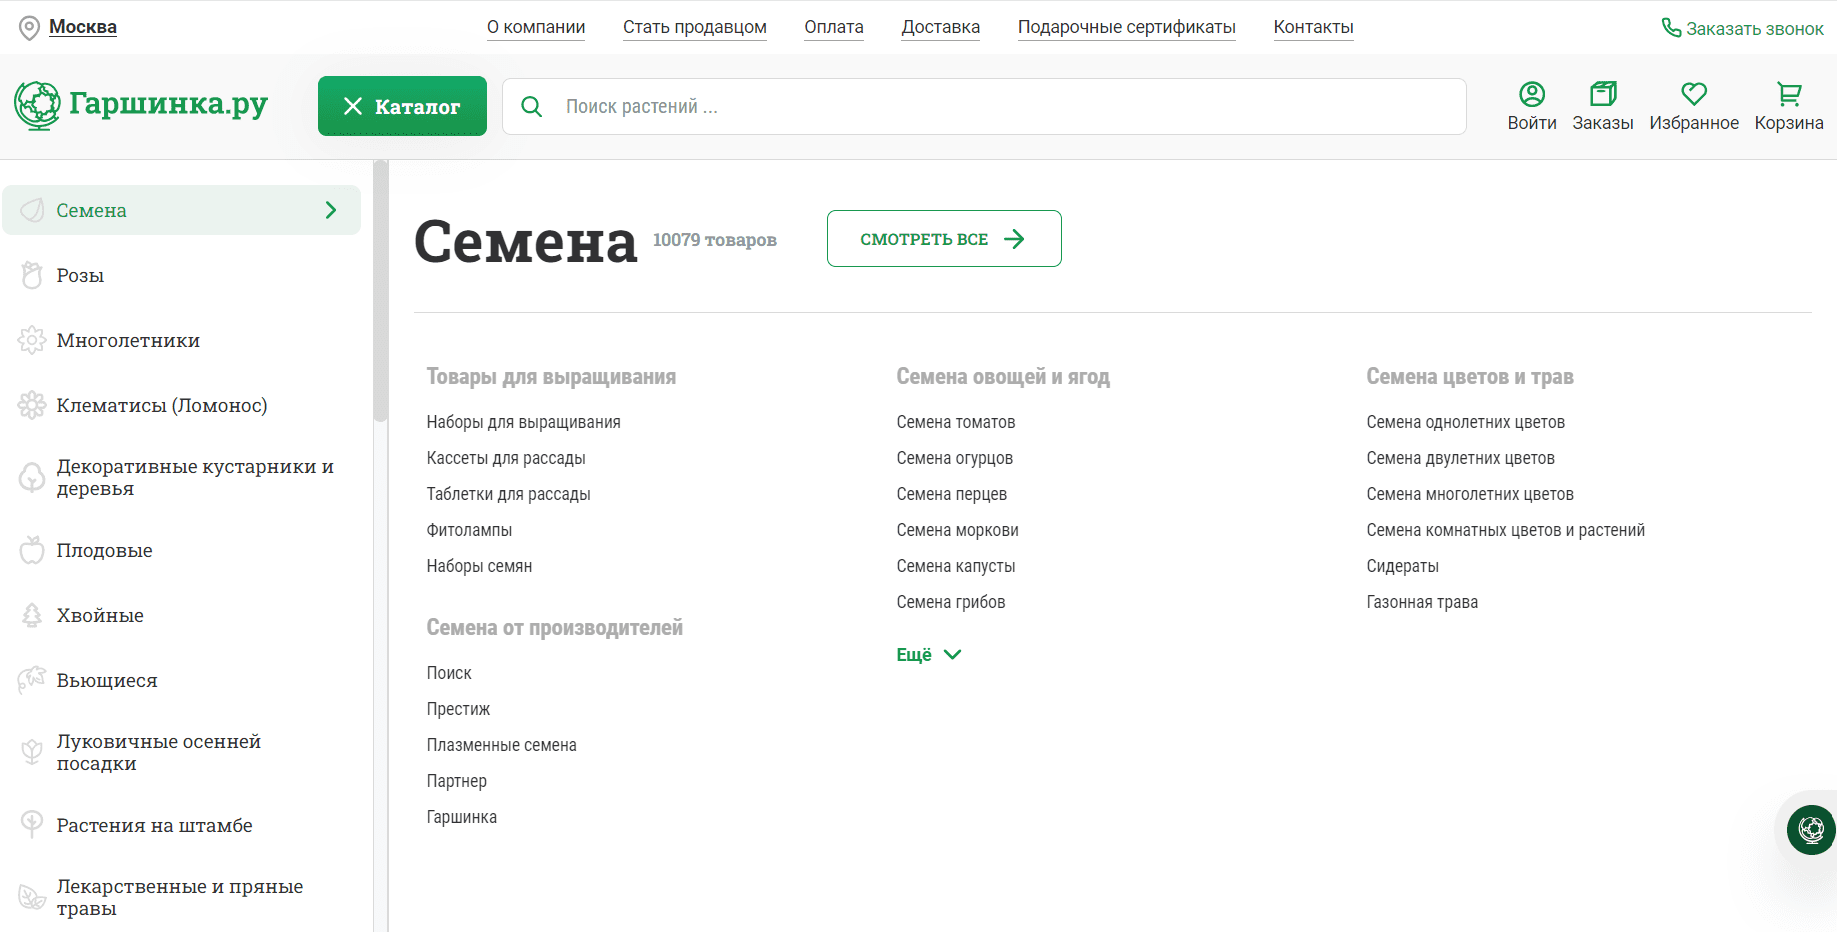
\includegraphics[width=0.8\linewidth]{garshinka}
	\caption{Каталог товаров магазина <<garshinka>>}
	\label{garshinka:image}
\end{figure}
%\vspace{-\figureaboveskip} % двойной отступ не нужен (можно использовать, если раздел заканчивается картинкой)


На рисунке ~\ref{pervocvet:image} представлен каталог товаров интернет-магазина <<pervocvet-shop>>.

\begin{figure}[h!]
	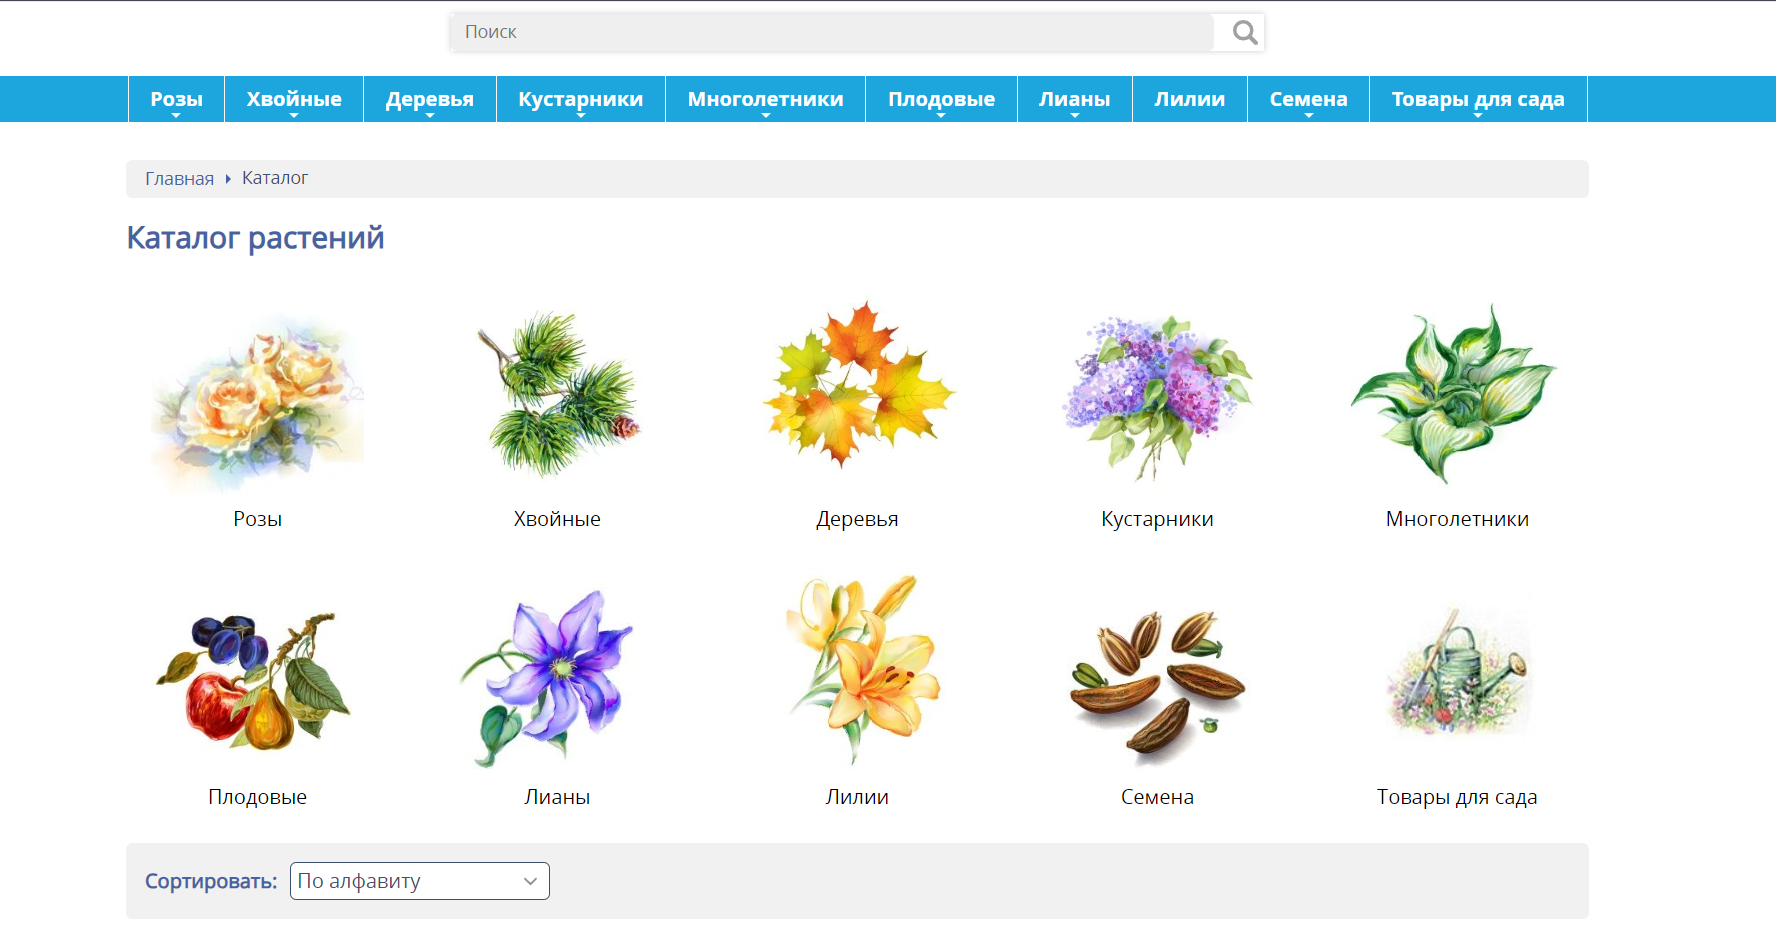
\includegraphics[width=0.8\linewidth]{pervocvet }
	\caption{Каталог товаров магазина <<pervocvet-shop>>}
	\label{pervocvet:image}
\end{figure}
%\vspace{-\figureaboveskip} % двойной отступ не нужен (можно использовать, если раздел заканчивается картинкой)


На рисунке ~\ref{plantmania:image} представлен каталог товаров интернет-магазина <<plantmania>>.

\begin{figure}[h!]
	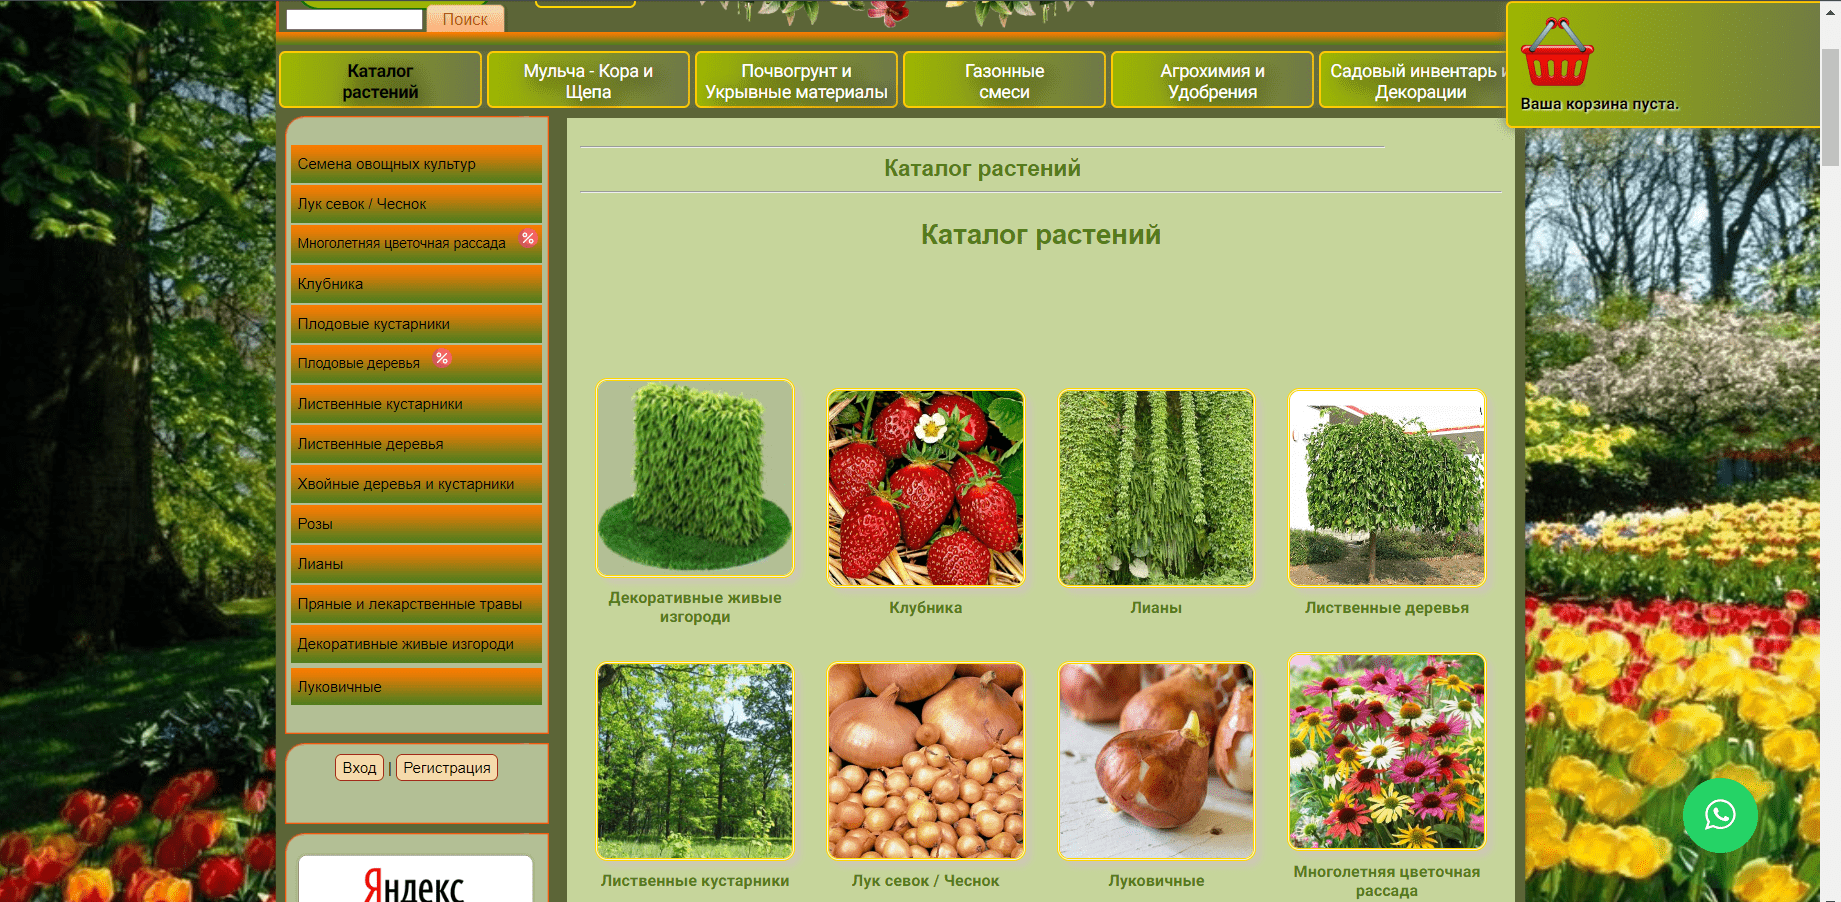
\includegraphics[width=0.8\linewidth]{plantmania}
	\caption{Каталог товаров магазина <<plantmania>>}
	\label{plantmania:image}
\end{figure}
%\vspace{-\figureaboveskip} % двойной отступ не нужен (можно использовать, если раздел заканчивается картинкой)


Каждый рассматриваемый магазин имеет категории, упрощающие поиск нужного товара. Можно заметить, что список категорий индивидуален для каждого сайта. Однако имеется общая черта: в список категорий входят разнообразные характеристики растений: жизненный цикл, тип посадочного материала и т.д. Причём, предлагаются не все варианты каждой характеристики: например, на каждом сайте имеется категория <<многолетние растения>>, но не представлены категории для двулетних и однолетних растений. Это позволяет пользователю без труда находить самые популярные категории,  но делает невозможным поиск для пользователя с более редкими требованиями.

Кроме того, все сайты имеют строку для поиска товара по названию, что является однозначным достоинством.

